% !TEX encoding = UTF-8 Unicode

%------------------------------------
%	PACKAGES AND OTHER DOCUMENT CONFIGURATIONS
%------------------------------------
\documentclass[letterpaper,11pt]{article}
\usepackage[utf8]{inputenc}
\usepackage[T1]{fontenc}
\usepackage{textcomp}
\usepackage{lmodern}
\usepackage[spanish,mexico]{babel} 
\usepackage{graphicx}
\usepackage{subcaption}
\usepackage{float}
\usepackage{blindtext}
\usepackage{fullpage}
\usepackage{amssymb}
\usepackage{mathtools}
\usepackage{algorithm}
\usepackage[noend]{algpseudocode}
\usepackage{nccmath}
\usepackage{enumerate}
\usepackage[none]{hyphenat}
\usepackage{amsmath}
\usepackage{graphicx}
\usepackage[table,xcdraw]{xcolor}
\usepackage{wrapfig}
\usepackage[colorinlistoftodos]{todonotes}
\usepackage[normalem]{ulem}
\useunder{\uline}{\ul}{}
\setlength{\parskip}{2mm}

\begin{document}

\begin{titlepage}

\newcommand{\HRule}{\rule{\linewidth}{0.5mm}} % Defines a new command for the horizontal lines, change thickness here

\center % Center everything on the page
 
%----------------------------------------------------------------------------------------
%	HEADING SECTIONS
%----------------------------------------------------------------------------------------

\textsc{\Large Universidad de Chile, Departamento de Ingeniería Eléctrica}\\[1.5cm] % Name of your university/college
\textsc{\Large Señales y Sistemas I}\\[0.5cm] % Major heading such as course name
\textsc{\large EL-3005-2}\\[0.8cm]
\textsc{\Large Proyecto 1}\\[0.5cm] % Minor heading such as course title

%----------------------------------------------------------------------------------------
%	TITLE SECTION
%----------------------------------------------------------------------------------------

\HRule \\[0.4cm]
{ \huge \bfseries Estudio de Técnicas de Procesamiento de Señales en Sistemas de Sonar}\\[0.1cm] % Title of your document
\HRule \\[1.5cm]
 
%----------------------------------------------------------------------------------------
%	AUTHOR SECTION
%----------------------------------------------------------------------------------------

\begin{minipage}{0.4\textwidth}
\begin{flushleft} \large
\emph{Autor:}\\
Felipe \textsc{Lucero}\\
19.528.232-3 % Your name
\end{flushleft}
\end{minipage}
~
\begin{minipage}{0.4\textwidth}
\begin{flushright} \large
\emph{Profesor:} \\
Jorge F. Silva
\\
[1.0cm]
\emph{Auxiliar:}\\
Roberto Rojas\\
\end{flushright}
\end{minipage}\\[2cm]

% If you don't want a supervisor, uncomment the two lines below and remove the section above
%\Large \emph{Author:}\\
%John \textsc{Smith}\\[3cm] % Your name

%----------------------------------------------------------------------------------------
%	DATE SECTION
%----------------------------------------------------------------------------------------

{\large \today}\\[2cm] 


\vfill 

\end{titlepage}

\newpage
\tableofcontents

\newpage

\section{Descripcion del Problema}

SONAR (\textit{\textbf{S}ound \textbf{N}avigation \textbf{A}nd \text{R}anging}) es una técnica de detección de objetos mediante el uso de ondas sonoras. El principio básico del SONAR se basa en la transmisión de una determinada señal acústica, y su posterior recepción debido a la reflexión de dicha onda con algún objeto en el ambiente. Formalente, considere $x_{a}(t)$ con $t$ $\in$ $\Re$, la señal transmitida e $y_{a}(t)$ la señal recibida dada por el siguiente modelo:

\begin{equation}
y_{a}(t) = \alpha(d)x_{a}(t-t_{d}) + w_{a}(t)
\label{modelo}
\end{equation}

Donde $|\alpha(d)| <  1$  denota la pérdida de energía de la señal emitida, $w_{a}(t)$ un ruido aditivo, $d$ la distancia al objeto y $t_{d}$ el tiempo que tomo la señal en ir y volver al emisor/receptor. Posteriormente, $x_{a}(t)$ e $y_{a}(t)$ son muestradas a una tasa $T_{s} = \frac{1}{F_{s}}$ acorde al toerema del muestreo, con el fin de procesar ambas señales y determinar el retardo temporal en la señal recibida. En consecuencia, las señales resultantes a tiempo discreto entán dadas por:


\begin{equation}
x(n) = x_{a}(nT_{s})
\end{equation}

\begin{equation}
y(n) = y_{a}(nT_{s}) = \alpha(d)x_{a}(nT_{s}-DT_{s}) + w_{a}(nT_{s})
\label{modelo2}
\end{equation}

\begin{equation}
= \alpha(d)x(n-D) + w(n)
\label{modelo3}
\end{equation}

donde $t_{d} \approx DT_{s}$. Finalmente, el problema consiste en determinar el retardo $D$ a partir de las señales $x(n)$ e $y(n)$.

\section{Desarrollo}

A continuación se describen una serie de análisis a realizarse con el objetivo de entender el procesamiento de las señales del SONAR.

\subsection{Relación con la correlación cruzada}

Como se planteó en las ecuaciones \eqref{modelo}, \eqref{modelo2} y \eqref{modelo3}, es de esperarse que la señal recibida $y_{n}$ sea muy parecida a $x(n)$, solo desplazada en D. Es decir, al realizar la correlación cruzada de las señales, se esperará un máximo en $r_{xy}(l)$ con $l$ muy relacionado con $D$.\par

Un ejemplo de esto se puede ver en las siguientes figuras:


\begin{figure}[H]
\centering
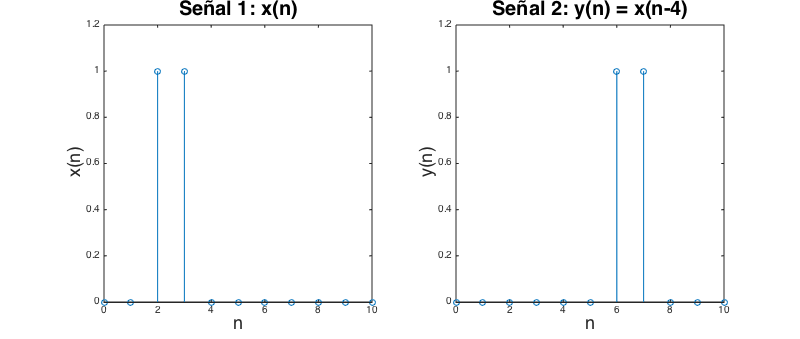
\includegraphics[width=1.0\textwidth]{img/parte_a/senales.png}
\caption{Dos señales, donde $y(n)$ es $x(n)$ desplazada en $k = 4$}
\label{desplazamiento}
\end{figure}

\begin{figure}[H]
\centering
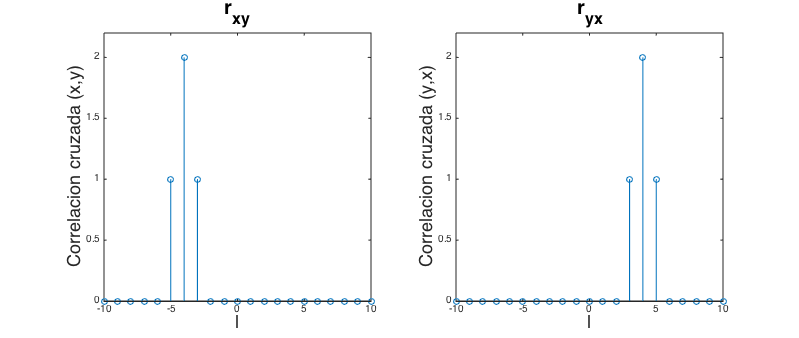
\includegraphics[width=1.0\textwidth]{img/parte_a/correlaciones.png}
\caption{Correlación cruzada entre las señales de la figura \ref{desplazamiento}, se aprecia el máximo en $l = \pm4$}
\label{correlacion}
\end{figure}

En la figura \ref{correlacion} se aprecia que el máximo se encuentra en $l = \pm 4$, que es justamente el desplazamiento relativo entre $x(n)$ y $y(n)$.

Con este análisis se puede corroborar que la técnica de la correlación cruzada es una buena técnica para encontrar el desplazamiento de la señal $D$.\par

Conociendo $D$, y utilizando la relación:

\begin{equation}
t_{d}\approx DT_{s}
\end{equation}

se podrá conocer el tiempo de retardo. Sabiendo que la velocidad de propagación del sonido en el mar es $ v = 1513 m/s$, se tendrá que:

\begin{equation}
d = \frac{vt_{d}}{2} \approx \frac{vDT_{s}}{2}
\end{equation}

Con esto explicado, se puede obtener la distancia al objeto

\subsection{Análisis a un set de datos conocidos}

Sabiendo el método para determinar la distancia, se puede aplicar esta técnica a datos conocidos. \par

Se considera una situación donde se emiten señales sonoras en todas direcciones ($360^{\circ}$), luego se reciben las señales, con ruido y perdida de energía.

La señal emitida es de tipo Gaussiana de la forma:

\begin{equation}
x_{a}(t) = \sqrt{\frac{20}{\sqrt{\pi}\sigma F_{s}}} exp\Bigg( -\frac{1}{2\sigma^2}(t-\mu)^2 \Bigg)
\end{equation}

donde $F_{s} = 5 kHz$ ,$\mu = 0.6s$ y $\sigma = 0.1s$

Se proporcionan 7 sets de datos $(Y_{k},Phi_{k})_{k=1...7}$, cada uno asociado a un entorno o escenario particular. Cada matriz $Y_{k}$ corresponde a la señal (de largo $N =10000$) para cada angulo (alrededor de 320, dependiendo del set de datos).\par

Con esto, se determina el entorno de la forma:

\begin{algorithm}[H]
\begin{algorithmic}
	\State $k \gets i \in (1..7)$
    \State Inicializar $x(n)$ como lista, funcion gaussiana
    
	\For{$Phi_{k}(i)$}
		\State $r_{i}$ = correlacion cruzada entre $Y_{l}(i,:)$ y $x(n)$
		\State $D_{i}$ = indice del máximo de r	
    \EndFor
    
    \State $distancia_{i}$ = velocidad$\cdot T_{s} \cdot D_{i}$ / 2
\end{algorithmic}
\end{algorithm}




Así se obtienene un arreglo de distancias para cada ángulo, obteniendo un par coordenado ($\phi_{k}$,$\rho_{k}$). Los resultados de este desarrollo, se encuentran en la siguiente sección.

\subsection{Respuesta segun la ganancia otorgada}

Naturalmente, se espera algun ruido adicional y una pérdida adicional de anergía a la hora de recibir la señal, como se aprecia en la ecuacion \eqref{modelo}, es por esto que es necesario algún tipo de amplificación, así la energía de la señal es superior y será más facil reconocerla. Si el ruido ambiente es mayor, entonces es necesario una mayor amplificación para obtener resultados útiles.\par

En este caso, la señal emitida será de la forma:

\begin{equation}
x_{G} = G\cdot x(n)
\end{equation}

Para simular la señal recibida, se utilizará la función preimplementada \texttt{data\_gen.m}, que simula parámetros como.

\begin{itemize}

\item $k$ : Ambiente a utilizar

\item $\sigma^2$ : Ancho de la señal emitida (varianza)

\item $\sigma_{w}^2$ : Varianza del ruido ambiente

\item $G$ : Ganancia de la señal

\end{itemize}

Para este informe, se utilizará $\sigma^2 = 0.01$ y $\sigma_{w}^2 = 50$ y se evaluará el desempeño de la técnica, según el valor de la ganancia $G$, para esto se utilizará el indicador ruido-señal:

\begin{equation}
\epsilon_{G,k} = \frac{||\hat{d}_{\phi,k} - d_{\phi,G,k}||_{2}}{||\hat{d}_{\phi,k}||_{2}}
\label{indicador}
\end{equation}

donde $d_{\phi,G,k}$ es un vector que posse la distancia detectada para cada angulo, en el escenario k, utilizando una señal transmitida con ganancia $G$, $\hat{d}_{\phi,k}$ son las distancias reales del escenario (conocidas) y $||x(n)||_{2} = \sqrt{\sum_{k} |x(k)|^{2}}$. Se generarán curvas $\epsilon_{G,k}$ vs $G$, para cada uno de los 7 escenarios posibles, con $G \in (0.5...90)$. Los resultados de este análisis se encuentran en la sección de resultados.


\subsection{Respuesta de la señal segun el ancho de la señal emitida}

En esta parte se estudiará el comportamiento o respuesta de la señal según el ancho de la señal $x(n)$ emitida.\par

En teoría, la respuesta de la señal debería depender de la frecuencia de la señal de incidencia, por una posible relación de dispersión en el mar y la forma de los objetos a detectar. Los componentes armónicos de la señal emitida (Gaussiana), dependen directamene de la varianza (ancho) de esta, por la Transformada de Fourier de una gaussiana (mientras más angosta, más componentes en frecuencia se necesitan), como se aprecia en la figura \ref{fourier}.\par

Análogamente a la subseccion anteriore utilizará nuevamente la función \texttt{data\_gen.m} para simular el escenario, esta vez variando $\sigma^2$ como parámetro de la forma $\sigma^2 = \{1,\frac{1}{2},\frac{1}{10},\frac{1}{20},\frac{1}{100},\frac{1}{200},...\}$ con $G = 1$ y $\sigma_{w}^2 = 0.5$ fijos.

También se utilizará un indicador ruido-señal, análogo al de la ecuacion \eqref{indicador}, donde se generaran curvas $\epsilon_{\sigma^2,k}$ vs $\sigma^2$ para cada escenario posible. Existirá un $\sigma^2$ óptimo para cada caso, donde se obtendrá el menor error. Los resultados de este análisis se encuentran en la siguiente sección.


\begin{figure}[H]
\centering
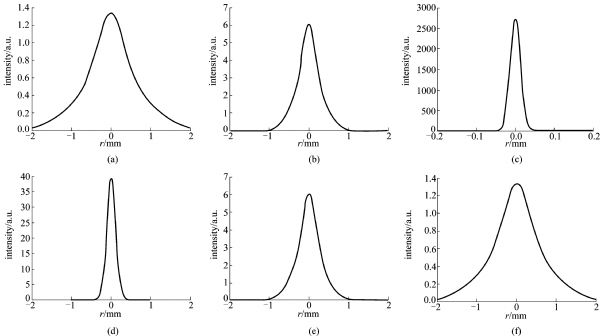
\includegraphics[width=1.0\textwidth,height = 0.45\textwidth]{img/parte_d/fourier.jpg}
\caption{Arriba: Señales continuas gaussianas con diferentes anchos. Abajo: Transformadas de Fourier para las gaussianas de arriba}
\label{fourier}
\end{figure}

\section{Resultados}

En esta sección se muestran los resultados para las pruebas y análisis descritos en la sección anterior.

\subsection{Análisis a un set de datos conocidos}
Llevando a cabo el algoritmo descrito en la sección anterior, se llega a los resultados de las figuras \ref{parteb1} y \ref{parteb2}.

\begin{figure}[H]
    \centering
    \begin{subfigure}[b]{0.3\textwidth}
        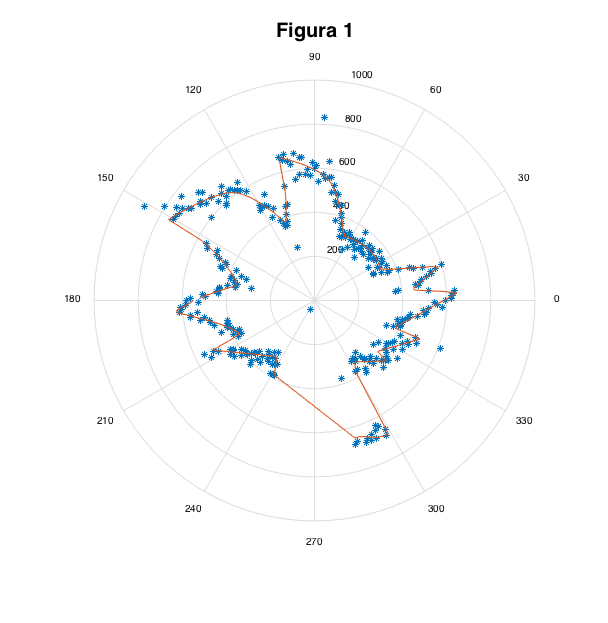
\includegraphics[width=\textwidth]{img/parte_b/figura1.png}
        \caption{Escenario 1}
    \end{subfigure}
    ~ %add desired spacing between images, e. g. ~, \quad, \qquad, \hfill etc. 
      %(or a blank line to force the subfigure onto a new line)
    \begin{subfigure}[b]{0.3\textwidth}
        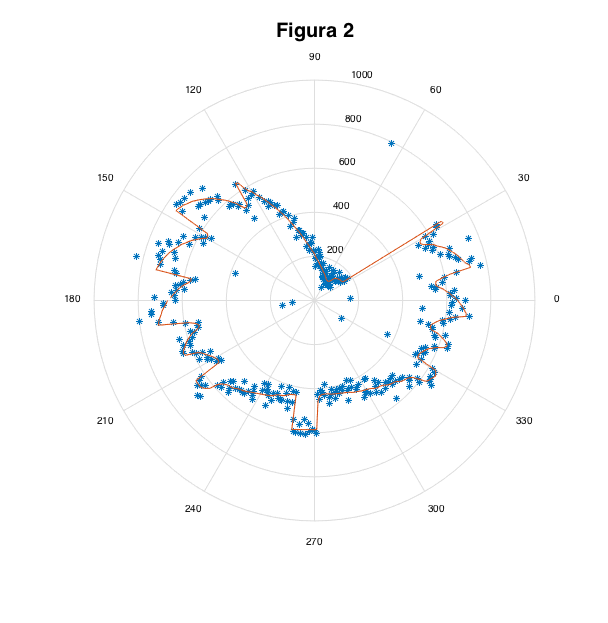
\includegraphics[width=\textwidth]{img/parte_b/figura2.png}
        \caption{Escenario 2}
    \end{subfigure}
    ~ %add desired spacing between images, e. g. ~, \quad, \qquad, \hfill etc. 
    %(or a blank line to force the subfigure onto a new line)
    \begin{subfigure}[b]{0.3\textwidth}
        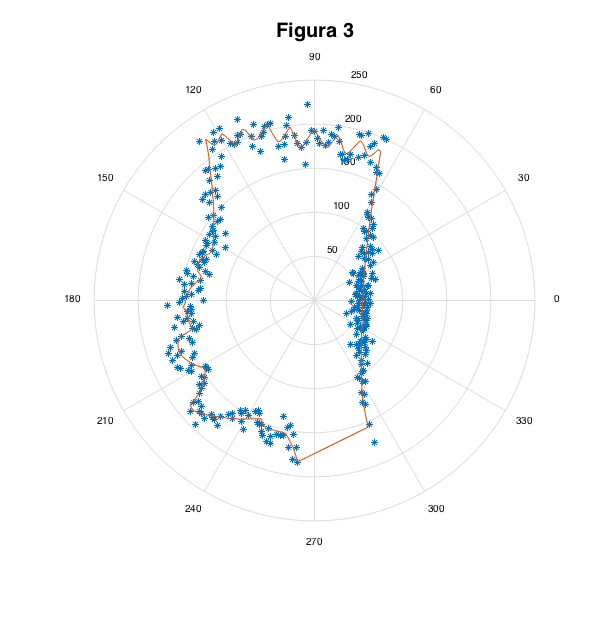
\includegraphics[width=\textwidth]{img/parte_b/figura3.png}
        \caption{Escenario 3}
    \end{subfigure}
    
    \caption{Puntos detectados para los tres primeros ambientes, utilizando la tecnica de la correlación cruzada}
    \label{parteb1}
\end{figure}


\newpage


\begin{figure}[H]
    \centering
        \begin{subfigure}[b]{0.45\textwidth}
        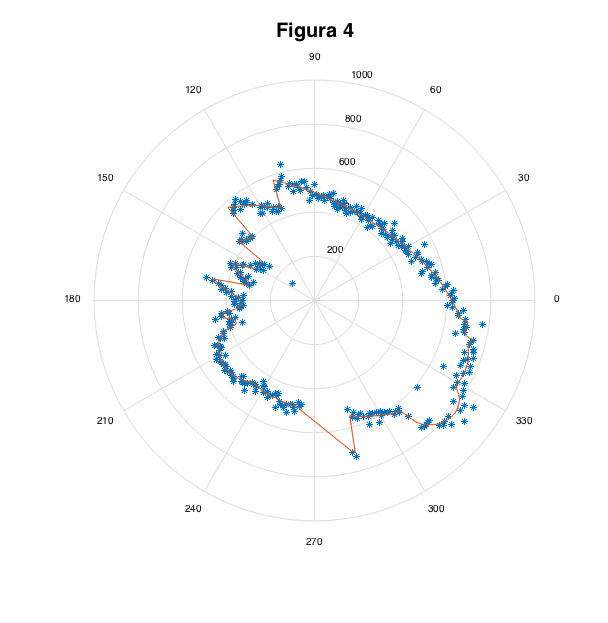
\includegraphics[width=\textwidth]{img/parte_b/figura4.png}
        \caption{Escenario 4}
    \end{subfigure}
    ~
    \begin{subfigure}[b]{0.45\textwidth}
        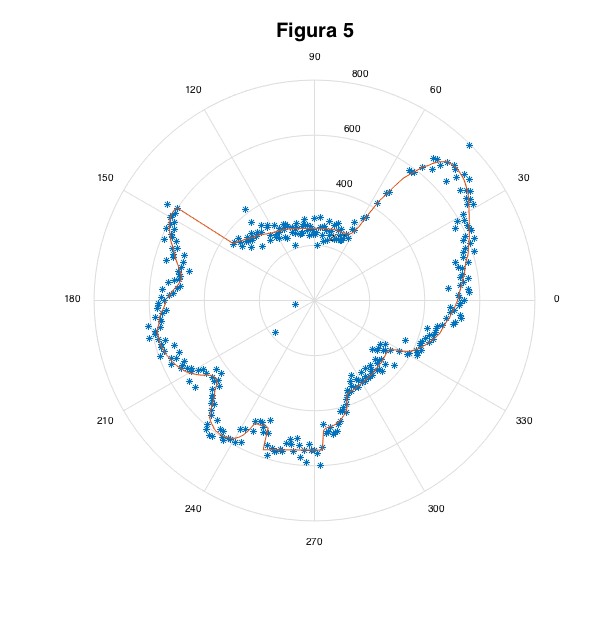
\includegraphics[width=\textwidth]{img/parte_b/figura5.png}
        \caption{Escenario 5}
    \end{subfigure}
    ~
    \begin{subfigure}[b]{0.45\textwidth}
        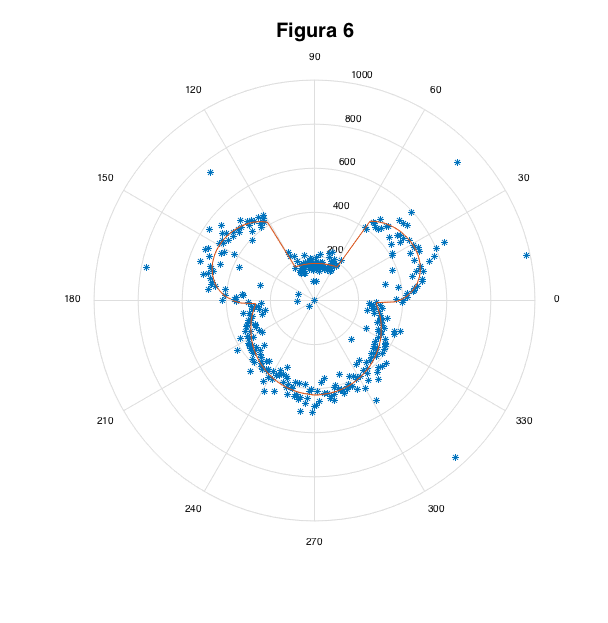
\includegraphics[width=\textwidth]{img/parte_b/figura6.png}
        \caption{Escenario 6}
    \end{subfigure}
    ~
    \begin{subfigure}[b]{0.45\textwidth}
        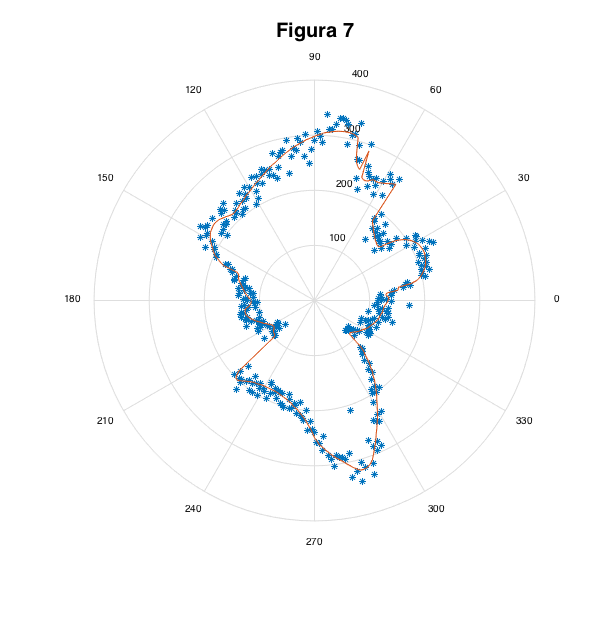
\includegraphics[width=\textwidth]{img/parte_b/figura7.png}
        \caption{Escenario 7}
    \end{subfigure}
    \caption{Resto de los entornos detectados utilizando la tecnica de la correlación cruzada}   
    \label{parteb2}
\end{figure}
   
Al ser datos de los cuales no se tenía ningun control (no se puede controlar la ganancia ni la varianza de la señal), es natural esperar algun ruido que distorsione la imagen (en naranjo se aprecia el entorno original).   


\subsection{Respuesta segun la ganancia otorgada}

Para las secciones siguientes, las pruebas requieren de un elemento aleatorio, por lo que los resultados no siempre serían los mismos, esto se puede compensar definiendo una semilla de random (siempre genera los mismos numeros aleatorios). En este caso se utilizó el comando \texttt{rng(42)}.

\begin{figure}[H]
    \centering
        \begin{subfigure}[b]{0.45\textwidth}
        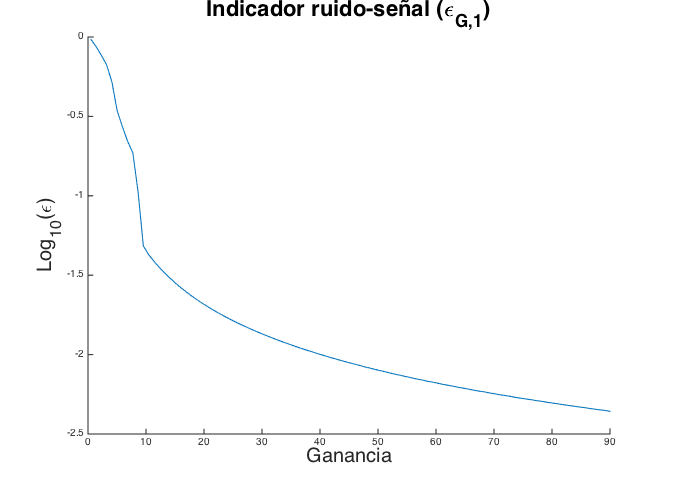
\includegraphics[width=\textwidth]{img/parte_c/curva1.png}
    \end{subfigure}
    ~
    \begin{subfigure}[b]{0.45\textwidth}
        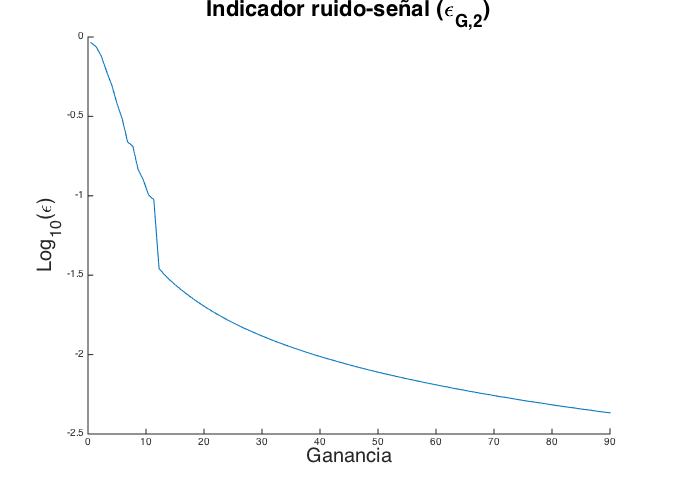
\includegraphics[width=\textwidth]{img/parte_c/curva2.png}
    \end{subfigure}
    ~
    \begin{subfigure}[b]{0.45\textwidth}
        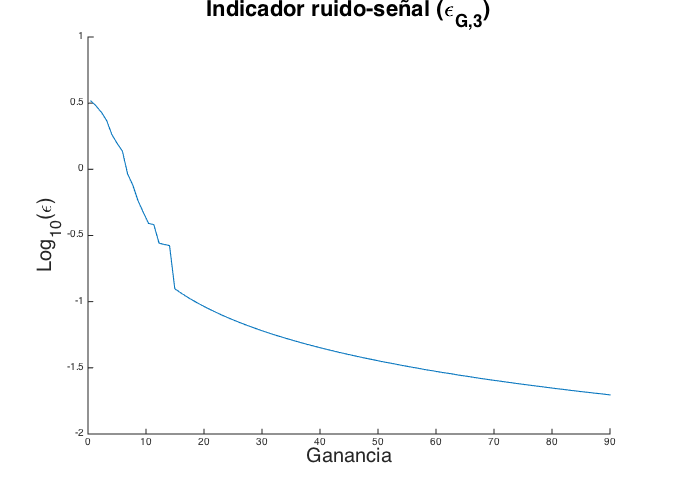
\includegraphics[width=\textwidth]{img/parte_c/curva3.png}
    \end{subfigure}
    ~
    \begin{subfigure}[b]{0.45\textwidth}
        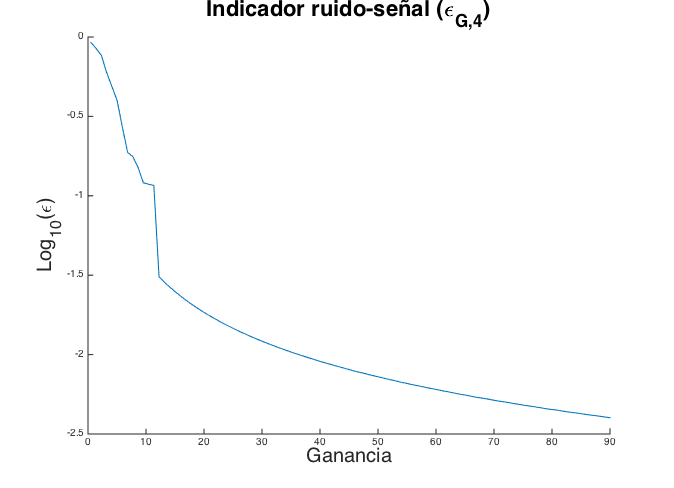
\includegraphics[width=\textwidth]{img/parte_c/curva4.png}
    \end{subfigure}
    \caption{Curvas $\epsilon_{G,k}$ vs $G$ para los 4 primeros entornos}   
    \label{partec1}
\end{figure}

Como es de esperarse, la curva es siempre decreciente, es decir $\epsilon_{G,k} \to 0$ cuando $G \to \infty$

\begin{figure}[H]
    \centering
    \begin{subfigure}[b]{0.3\textwidth}
        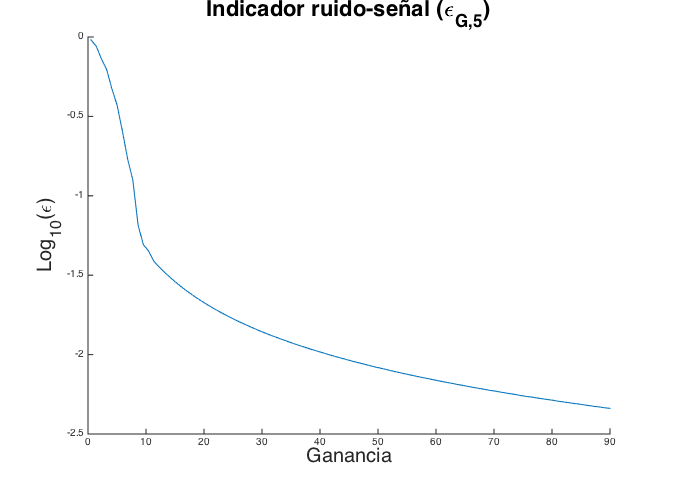
\includegraphics[width=\textwidth]{img/parte_c/curva5.png}
    \end{subfigure}
    ~ %add desired spacing between images, e. g. ~, \quad, \qquad, \hfill etc. 
      %(or a blank line to force the subfigure onto a new line)
    \begin{subfigure}[b]{0.3\textwidth}
        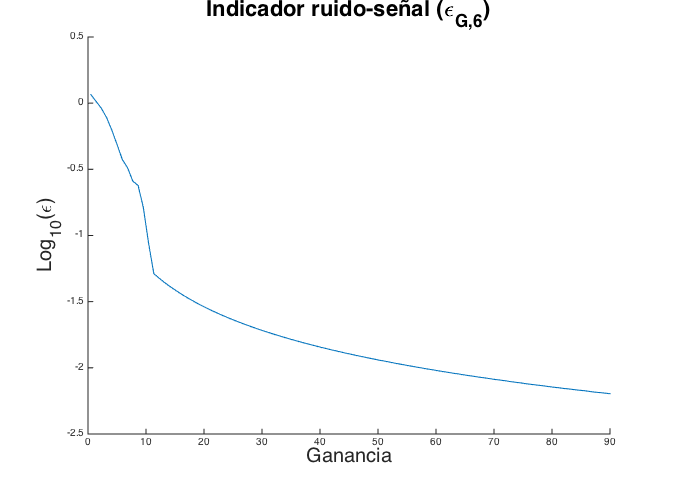
\includegraphics[width=\textwidth]{img/parte_c/curva6.png}
    \end{subfigure}
    ~ %add desired spacing between images, e. g. ~, \quad, \qquad, \hfill etc. 
    %(or a blank line to force the subfigure onto a new line)
    \begin{subfigure}[b]{0.3\textwidth}
        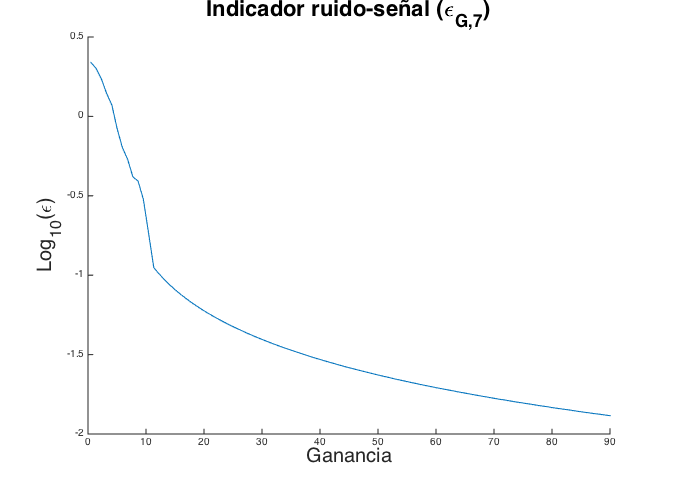
\includegraphics[width=\textwidth]{img/parte_c/curva7.png}
    \end{subfigure}
    
    \caption{Curvas $\epsilon_{G,k}$ vs $G$ para el resto de los entornos}
    \label{partec2}
\end{figure}

\begin{figure}[H]
    \centering
    \begin{subfigure}[b]{0.40\textwidth}
        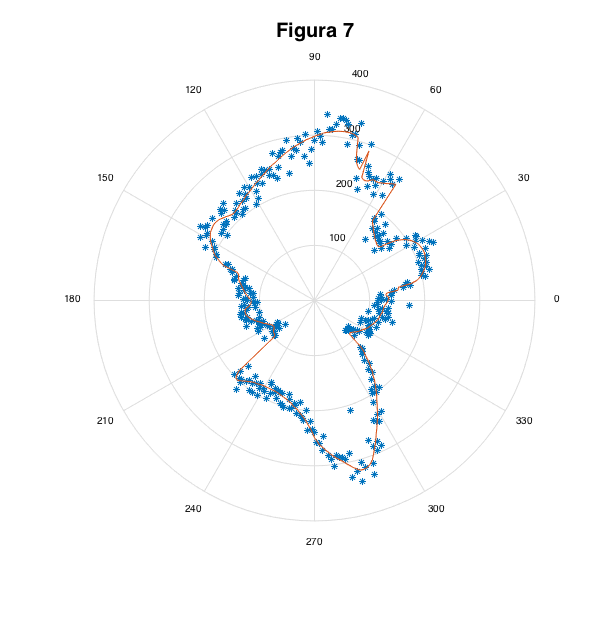
\includegraphics[width=\textwidth]{img/parte_b/figura7.png}
    \end{subfigure}
    ~ %add desired spacing between images, e. g. ~, \quad, \qquad, \hfill etc. 
      %(or a blank line to force the subfigure onto a new line)
    \begin{subfigure}[b]{0.45\textwidth}
        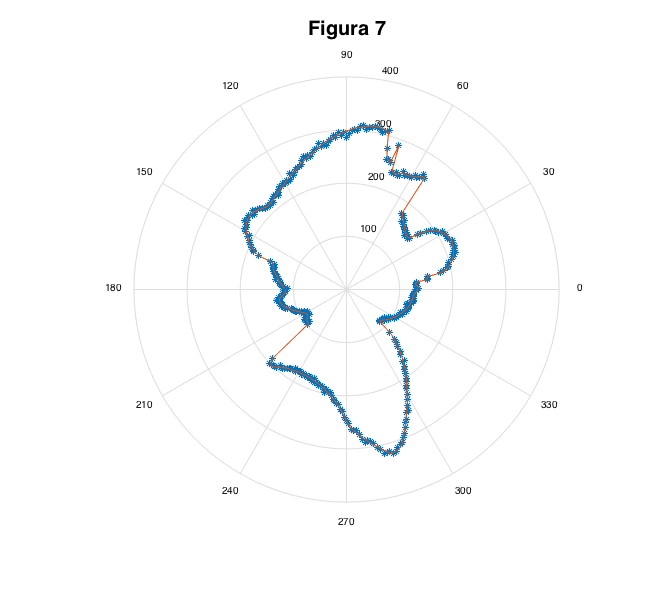
\includegraphics[width=\textwidth]{img/parte_c/figura72.png}
    \end{subfigure}
    
    \caption{Comparación de la detección de un entorno a diferentes ganancias}
    \label{partec3}
\end{figure}

\subsection{Respuesta de la señal segun el ancho de la señal emitida}

Al graficar el indicador $\epsilon_{\sigma^2,k}$ en primera instancia\footnote{Se grafica para el escenario 2, pero esto es arbitrario y para todos los entornos se obtiene un grafico de la misma forma.} se obtuvo un grafico como el de la figura \ref{error}.

\begin{figure}[H]
\centering
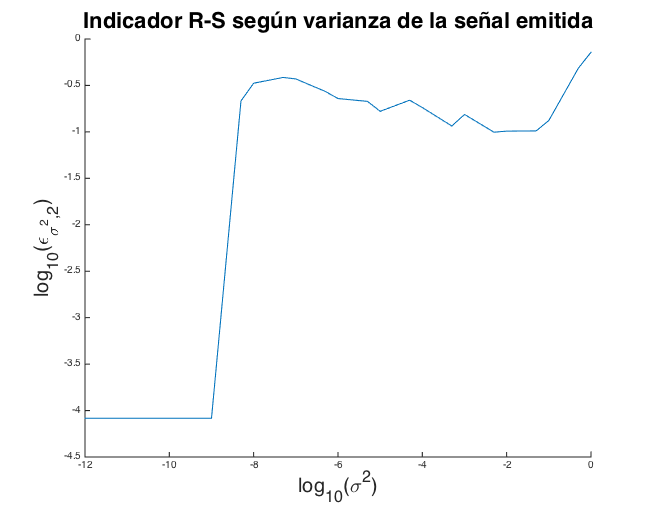
\includegraphics[width=0.7\textwidth]{img/parte_d/curvad2.png}
\caption{El indicador ruido-señal $\epsilon_{\sigma^2,k}$ vs $\sigma^2$, se aprecia una descontinuidad notoria en torno a $\sigma^2 \approx 10^{-9}$, en el entorno numero 2 (arbitrario)}
\label{error}
\end{figure}

Una posible explicación es que a medida que $\sigma^2 \to 0$, la señal Gaussiana se parece más a una función delta que tiende a infinito.

Esto implica que la energía de la señal ya no es constante y también tiende a infinito. haciendo un análisis incoherente pues se comparan señales con energía distinta, y como se vio anteriormente, una señal tiene respuestas distintas según la ganancia (eelacionada directamente con la energía). Esto queda más claro en la siguiente figura

\begin{figure}[H]
\centering
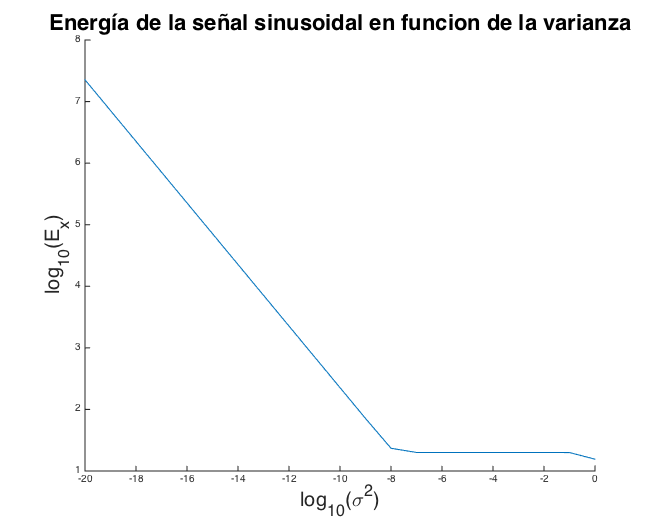
\includegraphics[width=0.7\textwidth]{img/parte_d/energia.png}
\caption{Energía de una señal gaussiana generada con \texttt{gaussian\_signal.m}, en función de la varianza $\sigma^{2}$, se aprecia un aumento de la energía en torno a $\sigma^{2} \approx 10^{-9}$}
\label{energia}
\end{figure}

Como se aprecia en la figura \ref{energia}, la energía ya no es constante cuando $\sigma^2 < 10^{-9}$, por lo que no tiene sentido buscar un optimo en el intervalo [0,$10^{-9}$].

Con esto dicho, en la figura \ref{error} se aprecia un óptimo para $\sigma^2$ en torno a $10^{-2}$ y es por esto que se buscara en el intervalo [$10^{-8}$,1].

Los resultados de esto se encuentran en la siguiente tabla:

\begin{table}[H]
\centering
\caption{óptimos y el indicador asociado para cada escenario}
\label{gaussiana}
\begin{tabular}{l|l|l|l|l|l|l|l|}
\cline{2-8}
                                                                      & \cellcolor[HTML]{C0C0C0}k = 1 & \cellcolor[HTML]{C0C0C0}k = 2 & \cellcolor[HTML]{C0C0C0}k = 3 & \cellcolor[HTML]{C0C0C0}k = 4 & \cellcolor[HTML]{C0C0C0}k = 5 & \cellcolor[HTML]{C0C0C0}k = 6 & \cellcolor[HTML]{C0C0C0}k = 7 \\ \hline
\multicolumn{1}{|l|}{\cellcolor[HTML]{C0C0C0}$\sigma^{2}_{ópt}$}      & $5\cdot 10^{-3}$              & $5\cdot 10^{-3}$              & $1\cdot 10^{-1}$              & $5\cdot 10^{-4}$              & $5\cdot 10^{-3}$              & $1\cdot 10^{-2}$              & $1\cdot 10^{-2}$              \\ \hline
\multicolumn{1}{|l|}{\cellcolor[HTML]{C0C0C0}$\epsilon_{\sigma^2,k}$} & 3.2 \%                        & 9.9 \%                        & 39.5 \%                         & 9.0 \%                        & 3.3 \%                        & 14.7 \%                       & 18.8 \%                       \\ \hline
\end{tabular}
\end{table}

Según esta tabla, existen ambientes mas propensos a resolverse mejor, el error mínimo es de $3.3 \%$ en el ambiente 1 y el máximo error es de $39.5 \%$ en el escenario 7.

Se compara la siguiente figura, se compara el peor escenario resuelto, con el mejor.


\begin{figure}[H]
    \centering
    \begin{subfigure}[b]{0.45\textwidth}
        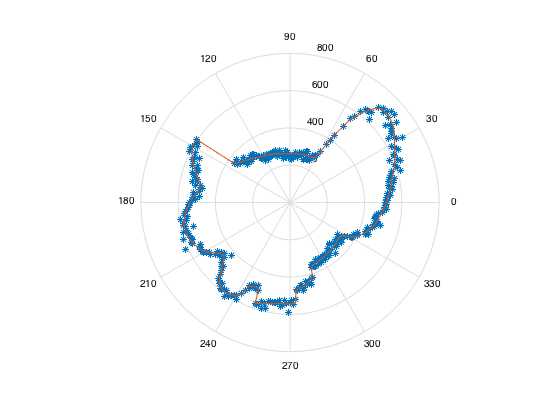
\includegraphics[width=\textwidth]{img/parte_d/mejor.png}
        \caption{Detección con minimo error}
    \end{subfigure}
    ~ %add desired spacing between images, e. g. ~, \quad, \qquad, \hfill etc. 
      %(or a blank line to force the subfigure onto a new line)
    \begin{subfigure}[b]{0.45\textwidth}
        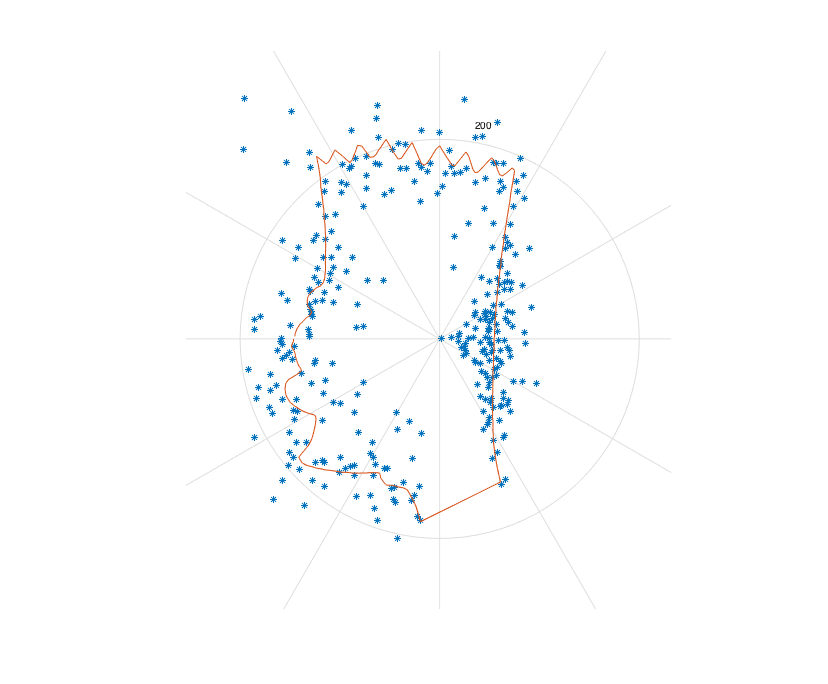
\includegraphics[width=\textwidth]{img/parte_d/peor.png}
        \caption{Detección con máximo error}
    \end{subfigure}
    \caption{Comparación para los optimos de $\sigma^2$ donde el error de la primera es de $3.3 \%$ y de la segunda es $39.5\%$}
    \label{parted}
\end{figure}


\subsection{Bonus: respuesta segun forma de la señal (pulso rectangular)}

En esta sección se comparan los óptimos de la sección anterior (Gaussiana), con un pulso rectangular, de la misma energía. Los optimos para este caso, donde $T$ es un parámetro que define el ancho del pulso rectangular se encuentran en la tabla \ref{pulso}.


\begin{table}[H]
\centering
\caption{Optimos del ancho para el pulso rectangular}
\label{pulso}
\begin{tabular}{l|l|l|l|l|l|l|l|}
\cline{2-8}
                                                               & \cellcolor[HTML]{C0C0C0}k = 1 & \cellcolor[HTML]{C0C0C0}k = 2 & \cellcolor[HTML]{C0C0C0}k = 3 & \cellcolor[HTML]{C0C0C0}k = 4 & \cellcolor[HTML]{C0C0C0}k = 5 & \cellcolor[HTML]{C0C0C0}k = 6 & \cellcolor[HTML]{C0C0C0}k = 7 \\ \hline
\multicolumn{1}{|l|}{\cellcolor[HTML]{C0C0C0}$T_{ópt}$}        & $5\cdot 10^{-1}$              & $1\cdot 10^{0}$               & $5\cdot 10^{-1}$              & $5\cdot 10^{-2}$              & $5\cdot 10^{-1}$              & $5\cdot 10^{-1}$              & $5\cdot 10^{-1}$              \\ \hline
\multicolumn{1}{|l|}{\cellcolor[HTML]{C0C0C0}$\epsilon_{T,k}$} & 7.6 \%                        & 10.2 \%                       & 51.0 \%                       & 10.7 \%                       & 6.3 \%                        & 13.4 \%                       & 25.9 \%                       \\ \hline
\end{tabular}
\end{table}

Se mantuvo constante la energía de la señal ($E_{x} =  20$) para poder realizar un análisis coherente.

Comparando las tablas \ref{gaussiana} y \ref{pulso} es apreciable que a gaussiana es más eficiente en la mayoría de los casos. Salvo en el escenario 6 que se observa en la figura \ref{bonusito}, donde practicamente no se aprecian diferencias notables.

\begin{figure}[H]
    \centering
    \begin{subfigure}[b]{0.45\textwidth}
        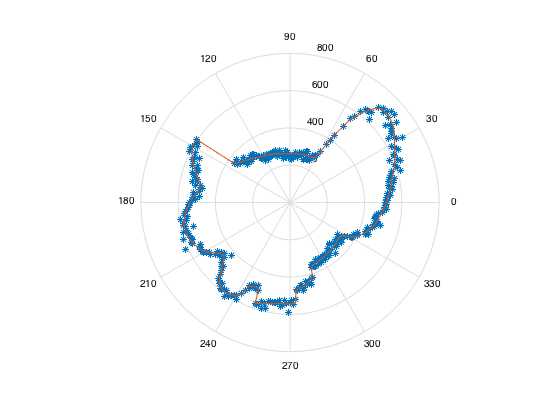
\includegraphics[width=\textwidth]{img/bonus/gaussian_signal.png}
        \caption{Detectado con señal gaussiana}
    \end{subfigure}
    ~ %add desired spacing between images, e. g. ~, \quad, \qquad, \hfill etc. 
      %(or a blank line to force the subfigure onto a new line)
    \begin{subfigure}[b]{0.45\textwidth}
        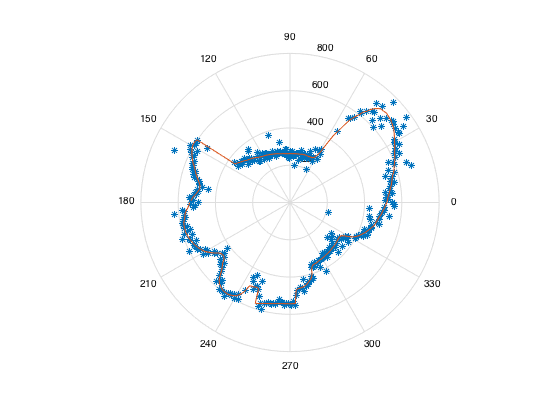
\includegraphics[width=\textwidth]{img/bonus/pulso.png}
        \caption{Detectado con pulso rectangular}
    \end{subfigure}
    \caption{Comparación de los óptimos para la señal gaussiana y el pulso rectangular, en el entorno 5.}
    \label{bonusito}
\end{figure}

\section{Análisis}

\subsection{Respuesta en función de la ganancia}

Recordando la ecuación \eqref{modelo}, si amplificamos la señal enviada por una ganancia $G$:

\begin{equation}
y_{a}(t) =\alpha(d) \big(G \cdot x_{a}(t-t_{d})\big) + w_{a}(t)
\end{equation}

Se tiene el termino $w_{a}(t)$ a la derecha, este término es independiente de la ganancia pues es el ruido ambiental y siempre está acotado por ciertos valores. Se puede aumentar sin perdida de generalidad la ganancia $G$ a tal punto tal que $w_{a}(t)$ sea despreciable, quedando un modelo de la siguiente forma:

\begin{equation}
y_{a}(t) \approx \alpha(d) \big(G \cdot x_{a}(t-t_{d})\big)
\end{equation}

es decir, el único factor que afecta a la señal\footnote{Este factor de atenuación es siempre necesario, ya que simula la perdida de energía por motivos físicos. Por ejemplo, es imposible detectar objetos si se encuentran a miles de kilómetros.} es $\alpha(d)$, y al realizar la correlación cruzada, se tendrán señales casi identicas y con muy poco ruido (siempre que la ganancia sea lo suficientemente alta).\par

Al encontrar el desplazamiento $D$, es muy probable que el error sea mínimo pues, como se mostró en la primera sección, la correlación cruzada encontrará el máximo en $D$.

Esto explica perfectamente el comportamiento decreciente de la curva $\epsilon_{G,k}$ vs $G$.

\subsection{Respuesta de la señal segun la varianza de la gaussiana emitida}

El óptimo para $\sigma^2$, que se aprecia en la figura \ref{optimo} puede ser explicado ya que, a medida que el ancho de la gaussiana disminuye, más es cercano a una función delta, haciendola confundible con el ruido exterior. \par

Una posible solución (si se buscara usar gaussianas más estrechas para más resolución\footnote{Por fenómenos ondulatorios, la resolución de los objetos detectados es directamente dependiente de la frecuencia utilizada. Por ejemplo, para detectar objetos pequeños se requieren longitudes de onda pequeñas, es decir, frecuencias altas. De todos modos, muy pocas veces se requiere encontrar objetos pequeños en el mar.}), es aumentar la frecuencia de muestreo así la señal, por muy estrecha que sea, será identificable como una gaussiana y será posible correlaciona y encontrar el desplazamiento. Esto está intimamente relacionado con el Teorema del Muestreo, pues al aumentar el ancho de banda, es posible detectar más componentes de frecuencia. 




\begin{figure}[H]
\centering
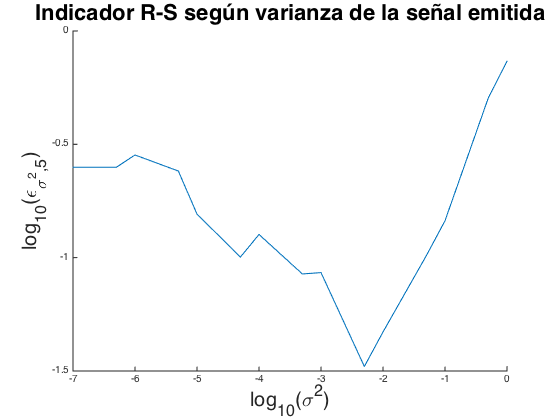
\includegraphics[width=0.7\textwidth]{img/parte_d/curva2d5.png}
\caption{El indicador ruido-señal $\epsilon_{\sigma^2,k}$ vs $\sigma^2$, se aprecia un error minimo para $\sigma^2$ en torno a $10^{-2}$, en el entorno numero 5 (arbitrario)}
\label{optimo}
\end{figure}


\subsection{Comparación de la señal gaussiana con un pulso rectangular}

Una explicación sencilla al porqué la señal gaussiana es más efectiva para detectar objetos es porque la señal cuadrada, al ser mas plana, es más facilmente confundible con el ruido exterior (al menos a la energía utilizada para el pulso). De todos modos es más fácil crear pulsos continuos (gaussiana).

\section{Conclusiones}

Del desarrollo de este informe y los análisis realizados, se pueden concluir los siguientes puntos:

\begin{itemize}

\item  El operador de correlación cruzada resultó fundamental para detectar desplazamientos a señales incluso siendo atenuedas por la distancia. Permite una complejidad a los algoritmos a utilizar que aumentan la efectividad y eficacia.

\item La implementación de la correlación cruzada en MATLAB usando la definición cruda, resultó muy ineficiente y lenta (aunque correcta). Existen métodos más rápidos que involucran el uso de FFT.

\item Claramente el ruido ambiente afecta considerablemente a la detección, esto es crucial si se trata de un barco (el ruido del motor o del barco desplazandose afecta). Sin embargo, en las secciones del informe se demostró que la amplificación ayuda a despreciar este problema.

\item Si se trata de naves militares por ejemplo, este tipo de sonar es inútil pues se revela la posición, o lugares donde no se quiera intervenir la fauna. Es por esto que existen sonares pasivos (que no emiten).

\item El ancho del pulso no es del todo determinante en estos casos simples, pues depende más del tipo de objeto a detectar (existian diferencias enormes entre un entorno y otro, en los óptimos). Para aumentar la eficacia es mejor amplificar la señal (con las consecuencias descritas en el punto anterior).

\item El tipo de pulso es más eficaz de tipo gaussiana (solo comparado con el pulso rectangular).

\item En otros casos, por ejemplo un pulso armónico (de una sola frecuencia), sería más util, pues por efecto Doppler se puede determinar además de la posición del objeto, la velocidad del objeto. Sin embargo en estos casos, la correlación cruzada perdería su utilidad (sirve desplazamientos temporales y no cambios en frecuencia).

\end{itemize}







\end{document}